%!TEX root = ../dissertation.tex
\chapter{Deep Neural Network}

In questo progetto viene utilizzata Convolutional Neural Network (CNN). Una descrizione completa delle NN si può trovare in \cite{Goodfellow-et-al-2016}, \cite[509-542]{journals/jasis/Biron97}, \cite[37-121]{Kriesel2007NeuralNetworks}. Le CNN verranno spiegate brevemente in seguito ma per maggiori dettagli si consulti \cite[326-365]{Goodfellow-et-al-2016}, \cite[106-119]{HabibiAghdam2017}.

Invece ci si vuole soffermare sulla spiegazione delle ottimizzazioni che vengono applicate alla rete. I due algoritmi principali sfruttati sono: l'algoritmo di Backpropagation e lo Stochastic Gradien Descent.

\section{Stochastic Gradient Descent}
Si prende $X$ per denotare un insieme di dati di training. Sarà conveniente considerare ogni input di training $\mathbf{x_i } \in X$ come un immagine e quindi con un vettore bidimensionale. L'output desiderato corrispondente è $\mathbf{y} = y(x)$, con $\mathbf{y}$ che invece rappresenta un vettore monodimensionale, i cui valori sono associati ciascuno ad ogni dato di input di training $\mathbf{x_i}$.
Si cerca un algoritmo che ci permetta di trovare pesi e bias in modo che l'output dalla rete si avvicini a $y( x )$ per tutti gli input di training $\mathbf{x_i}$. Per quantificare quanto bene si sta raggiungendo questo obiettivo viene definita una funzione di costo:

\begin{eqnarray}  C(w,b) \equiv
  \frac{1}{2n} \sum_x \| y(x) - a\|^2.
\end{eqnarray}

Qui, $\mathbf{w}$ denota la raccolta di tutti i pesi nella rete, $\mathbf{b}$ tutti i bias, $n$ è il numero totale di input di training, $\mathbf{a}$ è il vettore di uscite dalla rete quando $X$ è input, e la somma è su tutti gli input di training $\mathbf{x_i}$.
Ovviamente, l'output $\mathbf{a}$ dipende da $x$, $w$ e $b$, ma per mantenere la notazione semplice non viene indicata esplicitamente questa dipendenza. La notazione $|| \mathbf{v} ||$ denota semplicemente la norma di un vettore $\mathbf{v}$.

\'E chiamata C la funzione di costo quadratico. Ispezionando la sua forma si vede che $C( w,b )$ è non negativo, poiché ogni termine della somma è non negativo. Inoltre, il costo $C( w,b )$ diventa piccolo, cioè $C( w,b ) \approx 0$, precisamente quando $y( x )$ è approssimativamente uguale all'uscita, $a$, per tutti gli input di training, $x$.
Quindi l'algoritmo di training ha fatto un buon lavoro se è in grado di trovare pesi e bias in modo che $C( w , b ) \approx 0$. Al contrario, non sta andando così bene quando $C( w , b )$ è grande, questo significherebbe che $y( x )$ non è vicino all'uscita $a$ per un gran numero di ingressi. 
L'obiettivo dell'algoritmo di training sarà ridurre al minimo il costo $C( w , b )$ in funzione dei pesi e dei bias. Precisamente, si cercherà di trovare una serie di pesi e bias che rendano il costo il più piccolo possibile. E questo sarà possibile grazie ad un algoritmo noto come discesa del gradiente (Gradient Descent).
La funzione però riscontra dei problemi riguardanti la velocità di apprendimento, ma si è voluto introdurla perchè, utilizzando una funzione di costo uniforme come quella quadratica, risulta facile capire come apportare piccole modifiche nei pesi e nei bias in modo da ottenere un miglioramento nella funzione di costo. Quindi viene scelta una funzione di costo diversa, nota come Cross-Entropy. 

Si suppone di addestrare un neurone con diverse variabili di input,  $x1$, $x2$,… , corrispondenti ai pesi $w1$, $w2$,... e un bias, $b$. Un esempio è dato in Figura \textbf{\ref{fig:crossentropy}}.

\begin{figure}
\centering
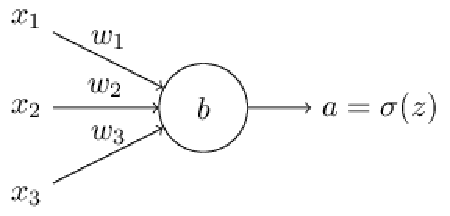
\includegraphics[width=%
0.5\textwidth]{figures/CrossEntropy}
\caption[Neurone Cross-Entropy.]{Rappresentazione di un neurone di bias $b$ con tre variabili di input $x_i$, ciascuna avente un peso $w_i$ e con output $\sigma(z)$.
\label{fig:crossentropy}}
\end{figure} 

L'uscita dal neurone è, naturalmente, $a=σ(z)$ , dove $z=\sum_j ( w_j * x_j ) + b$ è la somma ponderata degli input, mentre una descrizione completa della funzione di attivazione $\sigma$ la si può trovare in \cite[60-64]{Kriesel2007NeuralNetworks}.

Si definisce la funzione di costo Cross-Entropy per questo neurone come: %( Formula \textbf{\ref{form:costo}})

\begin{eqnarray} 
  C = -\frac{1}{n} \sum_x \left[y \ln a + (1-y ) \ln (1-a) \right]
%\label{form:costo}
\end{eqnarray}

Dove $n$ è il numero totale di dati di training, la somma è fatta su tutti i file di training, $\mathbf{x_i}$, e $\mathbf{y}$ è l'output desiderato corrispondente.

Minimizzare la funzione è un problema noto, ma non è di facile risoluzione in quanto ci sono molti fattori da considerare come la ricerca dei valori di $w$ e $b$ che minimizzano la funzione, il $\sigma$ funzione in background, la scelta dell'architettura di rete, i dati di input e così via. Il Gradient Descent è l'algoritmo che permetterà questa minimizzazione.

Nelle reti neurali spesso si hanno molte variabili, le reti neurali più grandi hanno funzioni di costo che dipendono da miliardi di pesi e bias in un modo estremamente complicato quindi usare il calcolo analitico per minimizzare non funzionerà. Viene sfruttata un'idea che sarà solo accennata in questa descrizione, vengono citati \cite{Goodfellow-et-al-2016} e \cite[91-94]{Kriesel2007NeuralNetworks} per approfondimenti sull' argomento. Si supponga di voler minimizzare la funzione in Figura \textbf{\ref{fig:vallevuota}}.

\begin{figure}
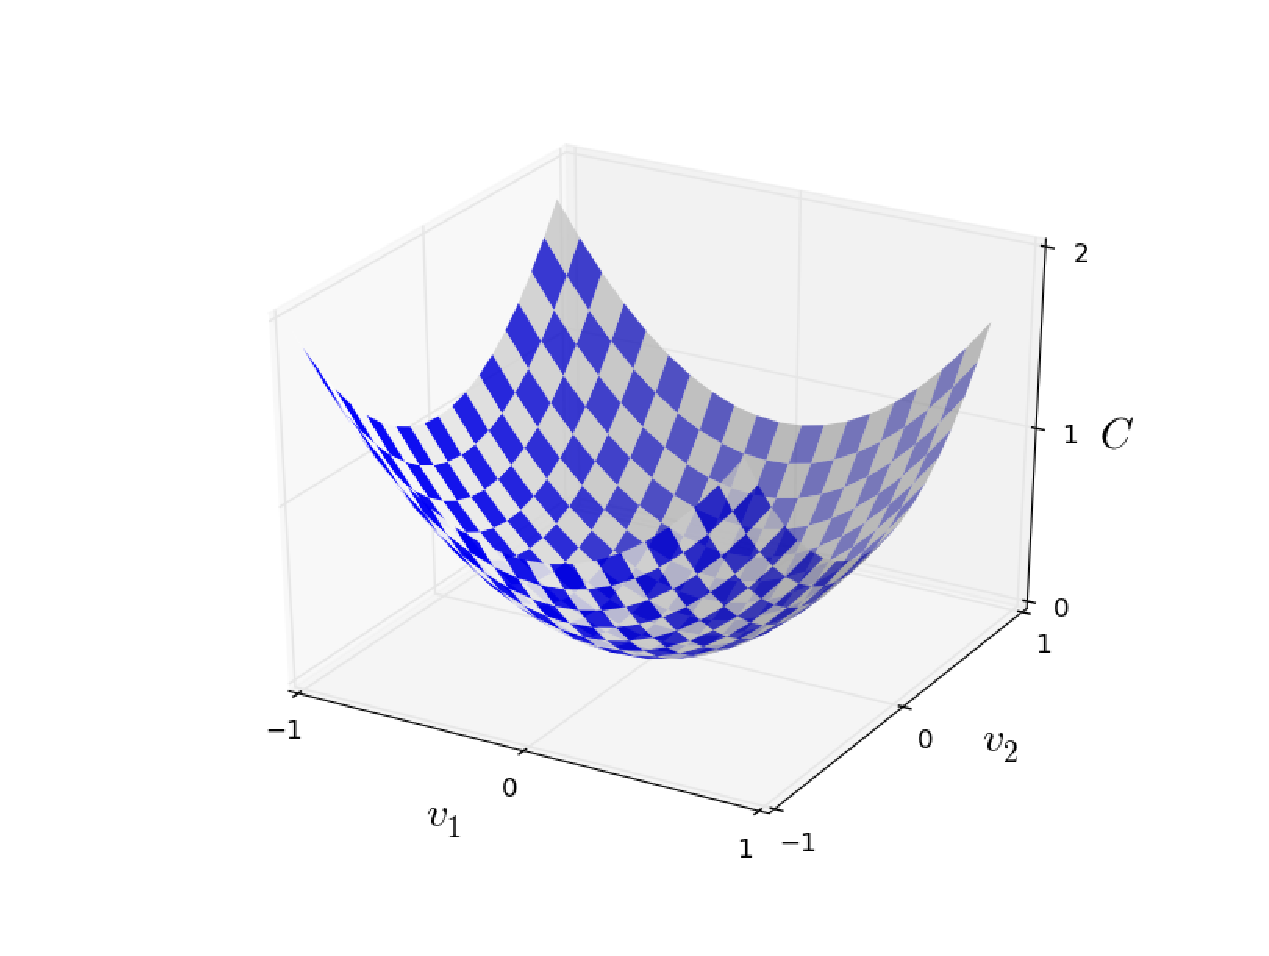
\includegraphics[width=%
0.8\textwidth]{figures/valley}
\caption[Funzione tridimensionale a forma di "valle".]{Funzione tridimensionale a forma di "valle".
\label{fig:vallevuota}}
\end{figure} 

\begin{figure}
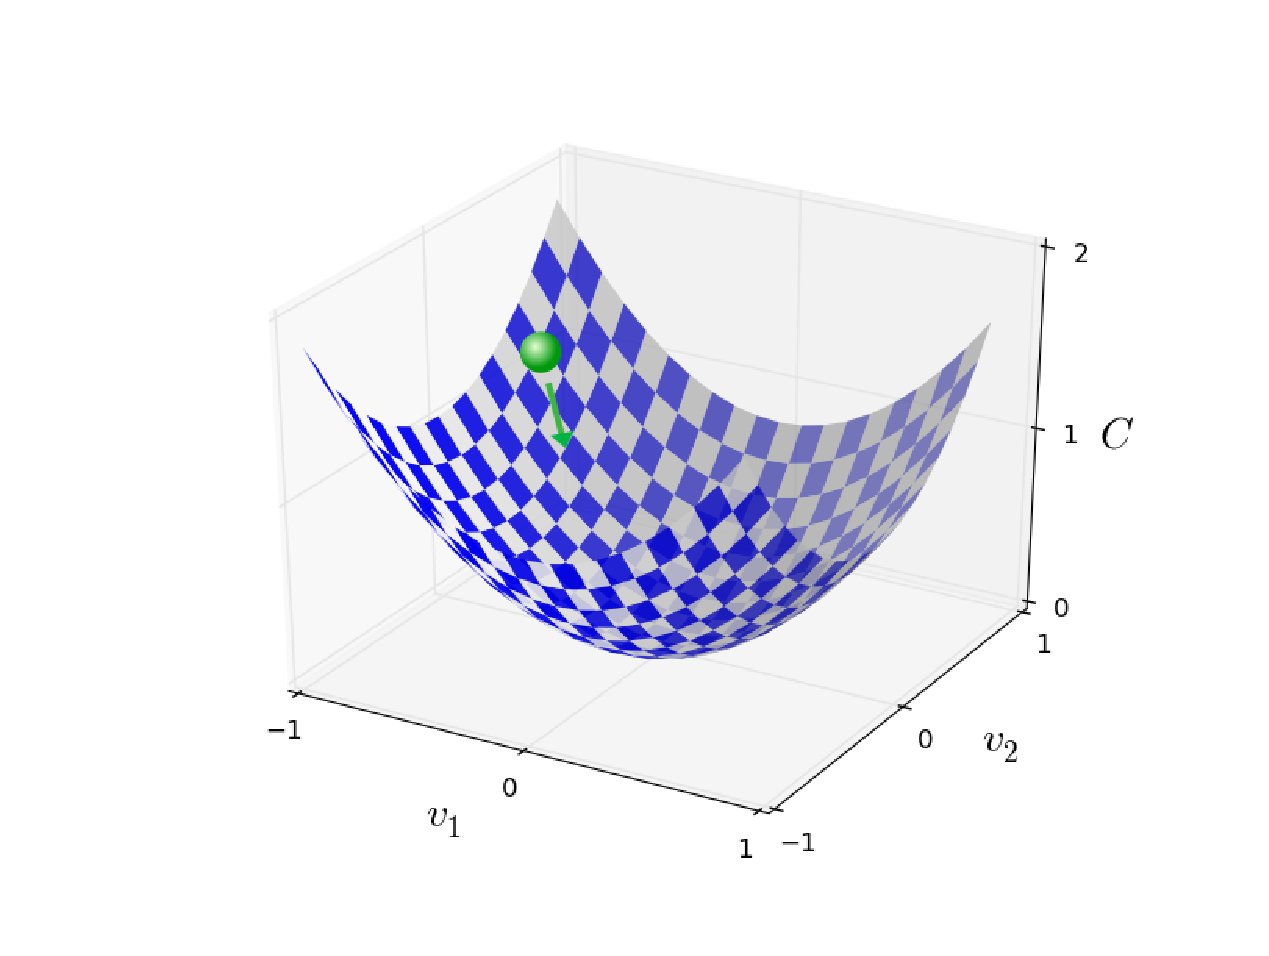
\includegraphics[width=%
0.8\textwidth]{figures/valley_with_ball}
\caption[Funzione a forma di "valle": Idea di minimizzazione]{Viene sfruttata l'idea fisica tale per cui se si lascia andare una palla da un punto della funzione, essa rotolerà verso il fondo e si fermerà solo quando avrà trovato il punto di minimo.
\label{fig:vallepalla}}
\end{figure} 

Uno dei metodi più banali per risolvere il problema è appoggiarsi ad una interpretazione fisica. Si immagini di prendere una sfera e di posizionarla in un punto qualasiasi della funzione, lasciandola liberà di muoversi come in Figura \textbf{\ref{fig:vallepalla}}. Man mano che essa farà uno spostamento verso il fondo della funzione, diminuirà anche la funzione di costo.
Quindi, il modo in cui l'algoritmo di discesa del gradiente funziona consiste nel calcolare ripetutamente il gradiente $\Delta C$, e quindi spostarsi nella direzione della pendenza della valle fino a raggiungere il punto minimo.
L'algoritmo non funziona sempre, diverse cose possono andare storte e impedire alla discesa del gradiente di trovare il minimo globale di C. Ma, in pratica, la discesa del gradiente spesso funziona molto bene, e nelle reti neurali è un modo efficace per ridurre al minimo la funzione di costo, aiutando così la rete ad apprendere.

\section{Algoritmo di Backpropagation}\label{sectionbackpropagation}
La Generalized Delta Rule \cite{rhw86}, nota anche come algoritmo di Backpropagation, viene introdotta per le Feed-Forward Neural Networks.

%WIKI{https://it.wikipedia.org/wiki/Rete_neurale_feed-forward} prime 5 righe
In queste reti neurali le informazioni si muovono solo in una direzione, avanti, rispetto ai nodi d'ingresso, attraverso nodi nascosti fino ai nodi d'uscita. Nella rete non ci sono cicli. Le reti feed-forward non hanno memoria di input avvenuti a tempi precedenti, per cui l'output è determinato solamente dall'attuale input.

%WIKI{https://it.wikipedia.org/wiki/Rete_neurale_artificiale}Storia
L'addestramento di une rete neurale con backpropagation avviene in due diversi stadi: forward-pass e backward-pass. Nella prima fase i vettori in input sono applicati ai nodi in ingresso con una propagazione in avanti dei segnali attraverso ciascun livello della rete (forward-pass). Durante questa fase i valori dei pesi dei neuroni sono tutti fissati. Nella seconda fase la risposta della rete viene confrontata con l'uscita desiderata ottenendo il segnale d'errore. L'errore calcolato è propagato nella direzione inversa rispetto a quella delle connessioni tra i neuroni. I pesi infine sono modificati in modo da minimizzare la differenza tra l'uscita attuale e l'uscita desiderata (backward-pass).

La spiegazione seguente è destinata a fornire una descrizione del processo coinvolto nell' algoritmo di backpropagation usando, per semplicità, una rete neurale contente 3 livelli. Questi sono: livello di input, hidden e di output.
Quindi, durante la fase di training (training phase), i dati di training (training data) vengono inseriti nel livello di input. I dati vengono propagati al livello hidden e quindi al livello di output. Questo è chiamato il passaggio in avanti dell'algoritmo di backpropagation (forward-pass). 
In questo passaggio, ogni nodo nel livello hidden ottiene input da tutti i nodi del livello di input, i quali vengono moltiplicati con pesi appropriati e quindi sommati. L'output del nodo hidden è la trasformazione non lineare della somma risultante. 
Allo stesso modo ogni nodo nel livello di output riceve input da tutti i nodi del livello hidden, che vengono moltiplicati con appropriati pesi e poi sommati. Nuovamente l'output di questo nodo è la trasformazione non lineare della somma risultante.
I valori di uscita del layer di output vengono confrontati con i valori di output di target, che sono quelli che si cercano di insegnare alla rete. L'errore tra i valori di output effettivi e i valori di output di target viene calcolato e propagato di nuovo verso il livello hidden. 
Questo è chiamato backward-pass della rete. L'errore viene utilizzato per migliorare la forza delle connessioni tra i nodi, ad es. le matrici di peso tra i livelli input-hidden e i livelli hidden-output vengono aggiornate.

Durante la fase di test, non avviene alcun apprendimento, ad esempio, le matrici di peso non cambiano. Ogni vettore di prova viene inserito nel livello di input. L'avanzamento (feed-forward) dei dati di test è simile a quello dei dati nella fase di training ma termina con i valori di uscita del layer di output. Un breve riassunto viene mostrato in Figura \textbf{\ref{fig:backpropagation}}\\

\begin{figure}
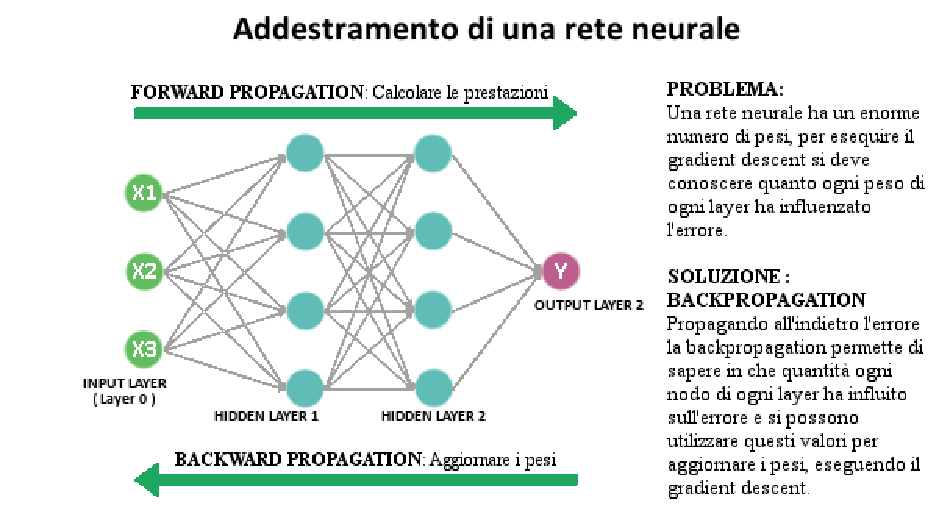
\includegraphics[width=%
1\textwidth]{figures/backpropagationsgd_mia}
\caption[Backpropagation]{Schema riassuntivo del funzionamento dell'algoritmo di Backpropagation in una rete neurale feed-forward.
\label{fig:backpropagation}}
\end{figure} 

\section{Convolution Neural Network}
Infine per la conclusione del capitolo si vuole lasciare una descrizione delle Convolutional Neural Networks (CNN) usate per questo progetto. Il loro nome deriva da una delle operazioni più importanti della rete: la convoluzione. Le CNN sono un tipo di rete neurale artificiale feed-forward in cui il pattern di connettività tra i suoi neuroni è ispirato dall'organizzazione della corteccia visiva animale.

La ricerca svolta negli anni '50 e '60 di D.H Hubel e T.N Wiesel \cite{Hubel1968} ha suggerito un nuovo modello per descrivere come i mammiferi percepiscono visivamente il mondo. Hanno mostrato che le cortecce visive di gatto e scimmia includono neuroni che rispondono esclusivamente ai neuroni nel loro ambiente diretto.
Nel loro articolo spiegano due tipi fondamentali di cellule del neurone visivo nel cervello che agiscono in modo diverso: cellule semplici (cellule S) e cellule complesse (cellule C).
Le celle semplici si attivano, ad esempio, quando identificano le forme base come linee in un'area fissa o un angolo specifico. Le celle complesse hanno campi recettivi più grandi e il loro output non è sensibile alla posizione specifica nel campo.
Le cellule complesse continuano a rispondere a un determinato stimolo, anche se la loro posizione assoluta sulla retina cambia.
Inoltre, il concetto di gerarchia gioca un ruolo significativo nel cervello. Le informazioni sono memorizzate come modelli, in ordine sequenziale. La neocorteccia, che è lo strato più esterno del cervello, immagazzina le informazioni gerarchicamente.

Nel 1980, Fukushima propose un modello gerarchico di rete neurale chiamato NeoCognitron \cite{Fukushima1980}. Questo modello fu ispirato dai concetti delle cellule semplici e complesse ed è stato in grado di riconoscere i modelli apprendendo le forme degli oggetti.

Più tardi, nel 1998, le CNN furono introdotte in un articolo di Bengio, Le Cun, Bottou e Haffner \cite{Lecun98}. La loro prima Convolutional Neural Network venne chiamata LeNet-5 ed era in grado di classificare cifre da numeri scritti a mano.\\

Tutti i metodi di riconoscimento degli oggetti all'avanguardia progettano le loro architetture di modelli attorno ad un concetto chiave per le CNN, il campo recettivo (Receptive Field).
Il campo recettivo è definito come la regione nello spazio di input influenzata da una particolare caratteristica di una CNN (Figura \textbf{\ref{fig:receptivefield}}). Un campo recettivo di una caratteristica può essere descritto dalla sua posizione centrale e dalle sue dimensioni. Tuttavia, non tutti i pixel in un campo sono ugualmente importanti per la caratteristica corrispondente della CNN. All'interno di un campo recettivo i pesi di ogni pixel vengono appresi dalla rete nella fase di training. In principio potrebbe apprendere che i pixel più lontani pesino di più anche se di solito, come in questo caso, più vicino è un pixel al centro del campo, più contribuisce al calcolo della funzione di output. Ciò significa che una caratteristica non guarda solo una particolare regione (cioè il suo receptive field) nell'immagine di input, ma si concentra anche verso la parte centrale di essa. 

\begin{figure}
\centering
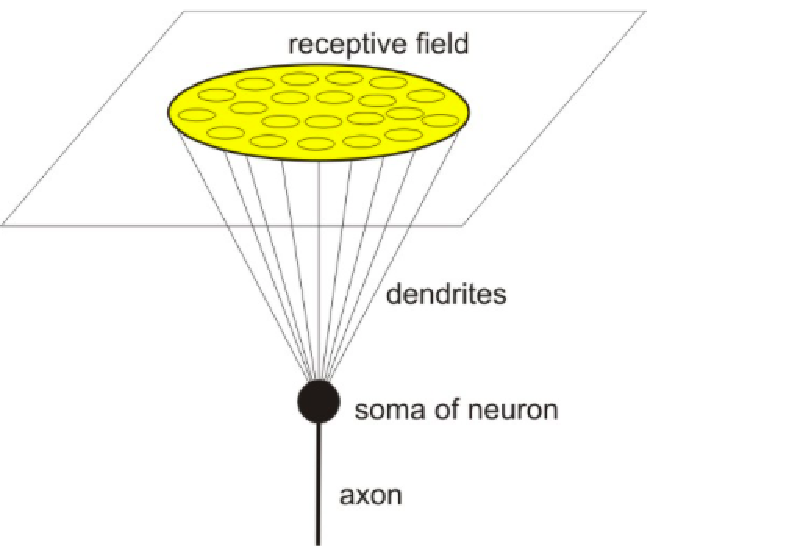
\includegraphics[width=%
0.5\textwidth]{figures/receptive_field}
\caption[Il Campo Recettivo di un neurone]{Il Campo Recettivo di un neurone - Sorgente: http://neuroclusterbrain.com/neuron\_model.html feed-forward.
\label{fig:receptivefield}}
\end{figure} 

In una CNN il campo recettivo può essere aumentato con metodi diversi, ad esempio: impilando più strati (profondità), Pooling (sottocampionamento), dilatazione del filtro, ecc. Tuttavia, ad esempio, impilando più strati è possibile aumentare linearmente il campo recettivo, ma in pratica non è così semplice in quanto aumenterebbe di conseguenza la complessità della rete e la difficoltà di allenarla, come dimostrato da Luo, Wenjie in \cite{NIPS2016_6203}.
La struttura delle CNN sarà spiegata in seguito nel Capitolo \textbf{\ref{strutturadellarete}}.
Per ulteriori studi si rimanda a \cite[326-366]{Goodfellow-et-al-2016} e \cite{Dumoulin2016AGT}.\\
% https://medium.com/mlreview/a-guide-to-receptive-field-arithmetic-for-convolutional-neural-networks-e0f514068807

\section{Struttura della rete neurale}\label{strutturadellarete}

La struttura e i moduli di base di una rete neurale convoluzionale sono: la convoluzione, il Pooling (Subsampling), la normalizzazione, il Fully Connected Layer e lo strato di apprendimento.

% SITO https://it.quora.com/Cos%E2%80%99%C3%A8-una-rete-neurale-convoluzionale
\subsection{Il processo di convoluzione} caratteristico di questo tipo di rete neurale, è ispirato dai processi biologici per l’analisi visiva negli organismi viventi. Lo strato di neuroni che si occupa della convoluzione divide l’immagine in vari frammenti sovrapposti, che sono in seguito analizzati per individuare le particolarità che lo caratterizzano, trasferendo l’informazione allo strato seguente sottoforma di una “feature map” contenente le relazioni tra neuroni e particolarità.

\subsection{Pooling} è un processo alquanto comune nelle reti neurali, che consiste nel generalizzare i dati per ridurne la dimensione, in modo da rendere più rapida l’analisi senza perdere troppa precisione. Nel caso di un’immagine, il processo è molto simile ad un sottocampionamento: una regione di pixel diventa un unico pixel al quale è assegnato un colore in base al massimo valore presente nella sua regione. (Figura \textbf{\ref{fig:maxpool}}).

\begin{figure}
\centering
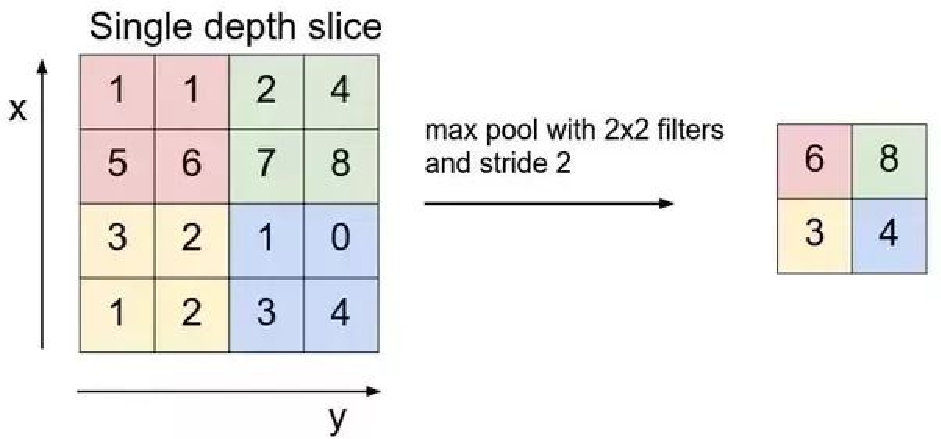
\includegraphics[width=%
0.8\textwidth]{figures/maxpooling}
\caption[Max Pooling.]{Il Max Pooling prende il valore più grande - Sorgente: \cite{CS231n}.
\label{fig:maxpool}}
\end{figure}

\subsection{La normalizzazione} è anch’essa largamente utilizzata per evitare le anomalie in seguito ai vari passaggi negli strati della rete neurale. Le funzioni più efficenti sono la Rectified Linear Units (ReLU), la tangente iperbolica e la fuzione sigmoide, anche se la ReLU è la migliore poichè più rapida ed evita il Vanishing Gradients. Viene rimandata la spiegazione a \cite{Goodfellow-et-al-2016} e \cite{Dahl2013}.

\subsection{Il Fully Connected Layer} nelle CNN rappresenta il vettore di caratteristiche per l'input. Questo strato di caratteristiche contiene informazioni molto utili per l'input. Quando la rete viene addestrata, esso viene utilizzato ad esempio per la classificazione, la regressione o l'input in altre reti, ecc. Durante la fase di allenamento, il fully connected layer determina la perdita e aiuta la rete a migliorare.
I livelli di convoluzione prima di esso contengono informazioni sulle caratteristiche locali dell'immagine di input quali bordi, blob, forme, ecc. Ogni strato di convoluzione contiene diversi filtri che rappresentano una delle caratteristiche locali. In questo progetto il fully connected layer è l'ultimo strato della rete e contiene le informazioni composte e aggregate da tutti i gli strati di convoluzione.

\subsection{Backpropagation} Infine, per le reti neurali c'è l'algoritmo di ottimizzazione che permette al sistema di modificare i pesi delle connessioni tra i neuroni sulla base della correttezza dei risultati emessi. Il metodo utilizzato è la Backpropagation spiegata nella sezione precedente (\textbf{\ref{sectionbackpropagation}}).